
\section{Motivation}
Empirical measurements are critical tasks to capture the effect of developers' choice on software energy consumption.
To accomplish this, one should not overlook the benchmarking pitfalls highlighted in the state of the art.
Moreover, when it comes to measuring the energy consumption of software, other obstacles arise, such as the impact of hardware, the difference between the machines used for measurements purpose and the ones that may apply the findings, etc. 
Moreover, significant improvements in computer science have resulted in an increase in the quantity of obsolete results.
It is even more difficult to address all of them in studies that compare multiple solutions.
Furthermore, there may have been the appearance of new candidates, as well as the development of others between the preliminary experiment and the published results.
As a result, it is not only required to ensure the "reproducibility" of the results, but also to make way for new candidates.
Hence, we would like to propose a new concept to leverage experiments, which we call "Extension".
The capacity to provide the tools required not only to repeat the experiments, but also to include additional candidates, workloads, or relevant key performance indicators.

This chapter discusses how to solve the challanges of empirical analysis when it comes to the energy consumption experiments,

first we will dicuss how to ensure the three aspects of successful benchmark within the energy consumption. 
So section~\ref{sec:benchmarking_reproducibility} will focus on the "reproducibility" aspect and how to provide reproducible experiments without impacting the energy measurement. 
Section~\ref{sec:taming-the-energy-variation} will be about the accuracy when it comes to software energy consumption. and finally 
Section~\ref{sec:extension} will be about the tools to include new candidates, workloads, or relevant key performance indicators. 

As for "representativeness" of the benchamrks, we will discuss it further in the Perspectives section.
 
%% this is might be the part that treats reproducibility for my case 



%%%%%%%%% preliminary taughts and section structure 
% The need of reproducibility in our field - software optimization based on empirical studies -

% The importance of Virtualisation for reproducibility \cite{howe_virtual_2012}
% some of the most important parts are
% - fewer constraints on research methods
% - on-demand backups
% - virtual Machines as Publications
% - more Variables captured



%%%% part of the state of the art 
% In the area covered by this PhD thesis, reproducibility might be achieved by ensuring the same execution settings of physical nodes, virtual machines, clusters or cloud environments.
%%% why it won't work for energy consumption 
% However, when it comes to measuring the energy consumption of a system, applying acknowledged guidelines and carefully repeating the same benchmark can nonetheless lead to different energy footprints not only among homogeneous nodes, but even within a single node.
%% reseasons why 
% One major problem that hinders the reproducibility of the empirical benchmarks is the interaction with the external environment, either as concurrency or dependencies.
% Therefore, researchers cannot observe the same results, unless they duplicate the same environment.


% \begin{itemize}
%     \item textbf{expermimental protocol}: Which describes, the context and  an orchestrator that handles the experiment, this orchestrator should take as an entry 
%     \item \textbf{candidates}: a set of candidates that will be used in the experiment. The candidates should be agnostic of the experiment context and they all
% \end{itemize}
\section{Reproducibility within the context of energy}\label{sec:benchmarking_reproducibility}
% Now that we have covered the general strucutre of the protocol, this section details the specific aspects of the protocol that are relevant to the energy consumption analysis.
% We will first discuss how to insure the extension of the candidates. later we will talk about the energy metrics and how to ensure the accuracy when it comes to the measurement of the energy consumption.
This section thus discusses different ways to enforce the reproducibility of experiment by comparing different ways to encapsulate the systems-under-test.

\paragraph{Virtual Machines}
First option should be using \emph{Virtual Machines} (VM), which gives researchers the freedom to choose the most appropriate tools, software and operating system that they are the most comfortable with, without paying the price to change the actual working environment, which will give them eventually more control over the dependencies and the execution environment.Therefore, Adding a new candidate is as simple as adding a new VM to the experiment.
Moreover, using a VM addresses the \emph{replication crisis} thanks to the virtual images, as even the most complex architecture can be reproduced easily by instantiating a copy of the image. 
However, this choice comes with a certain cost.
Because of the hypervisor, software will build on two kernels---the virtual machine (guest) one and the host machine one---which will provide a noticeable overhead, and will impact the performances of the system-under-test.
Therefore, we cannot use VM for experiments that are related to performance.
Another limitation of VM is the the isolation.
While this feature prevents the experimental environment from any undesirable interference from the outside world, this interaction may be required---especially when the experiment is dependent to an external 

\paragraph{Containers}
Another solution would be using something that allows us to benefit from the isolation of the host OS, while easing of replication proposed by VM, and the direct interaction with the hardware that the classical method give.
Containers offer such an advantage, while ensuring the isolation and the ease of replication for application.

Figure~\ref{environement:virtualization_technique} explains the differences in architecture between the types of virtualization and container technologies:
\begin{itemize}
    \item \textsf{Type\,1} runs directly on the hardware, it is mainly used by the cloud providers where there is no host OS, but just VM, use the open-source Xen or VMware ESX hypervisors to be executed;
    \item \textsf{Type\,2} runs over the host OS, mostly used for personal computers.
    VMware server and virtualBox are popular examples of this type, and most of the researchers experimentation are run with this type. However, due to the 2 OS, the applications tend to be slower.
    \item \textsf{Containers}. Instead of its own kernel, containers use the host kernel to run their OS, which makes them lighter, faster and use the full potential of hardware.
    For this category, one can cite \emph{Docker}, \emph{Linux LXC}, or \emph{LXD}~\cite{abuabdo_virtualization_2019}.
\end{itemize}


\begin{figure}
    \center{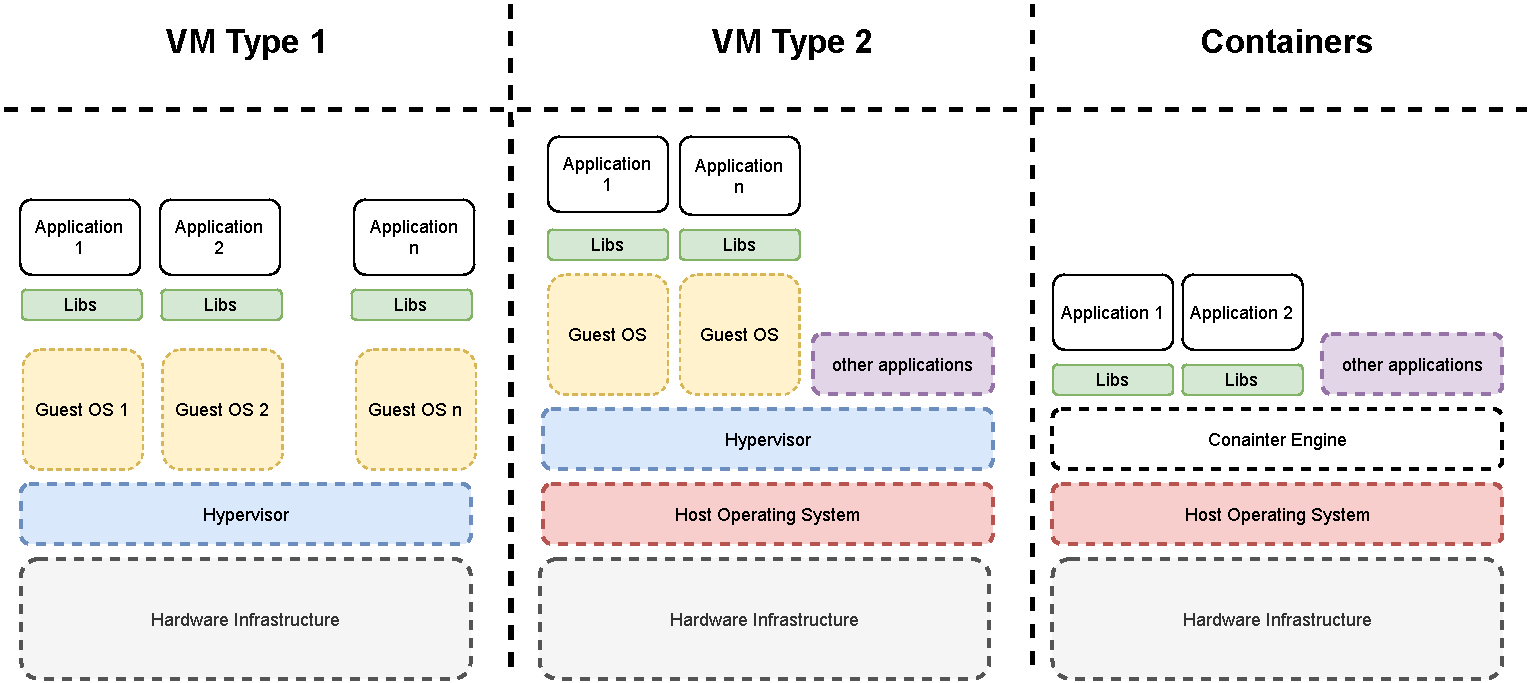
\includegraphics[width=1\linewidth]{imgs/virtualization_techniques}}
    \caption{Different Methods of Virtualization}\label{environement:virtualization_technique}
\end{figure}


\subsection{Docker Vs. Virtual Machine}
Despite the fact that \textsf{Type\,1} is more performant than \textsf{Type\,2}, the second one is the most used in research, as most researchers tend to conduct their experiments in their own machine.
In the other hand, Docker is the most famous container technology.
In our case, we are more prone to promote Docker for two reasons:
\begin{enumerate}
    \item we need a lightweight orchestrator to limit the overhead on energy consumption of our tests, as prior work mentioned
    \cite{van2016power}
    % TODO : ask romain about the title of the paper and the reference to the paper
    [cite Morabito (2015) and van Kessel et al. (2016)],
          % cite Power efficiency of hypervisor-based virtuali- zation versus container-based virtualization. University of Amsterdam.
    \item as we are using hardware sensors to measure the energy consumption, we need to interact with the host OS.
\end{enumerate}

Special notice to \href{https://github.com/powerapi-ng/virtualwatts}{virtualwatts}. A framework that allows us to retireve the energy consumption of a virtual machine.


\subsection{Docker \& Energy}
Now that we have chosen to go with the containers technology to encapsulate our tests.
What would be the impact of this solution on the energy consumption of our tests.

Based on the studies of \cite{santos2018does}, who analysed the impact of adding the Docker layer on the energy consumption.
In their experiment, Eddie Antonio~\emph{et~ al.} run multiple benchmarks with and without Ddocker. 
They compared the resulting energy consumption and execution time.
The first step was to see the impact of Docker deamon, while there is no work, to observe the impact of the orchestrator.
Then, they conduct their experiments with the following benchmarks:
\begin{itemize}
    \item Wordpress,
    \item Reddis,
    \item PostgreSQL.
\end{itemize}

The following figures represents the energy consumption of the system-under-test while it is idle.
As one can observe in Figure~\ref{fig:docker_idle}, Docker brings an overhead of around $1,000$ Joules.

\begin{figure}
    \center{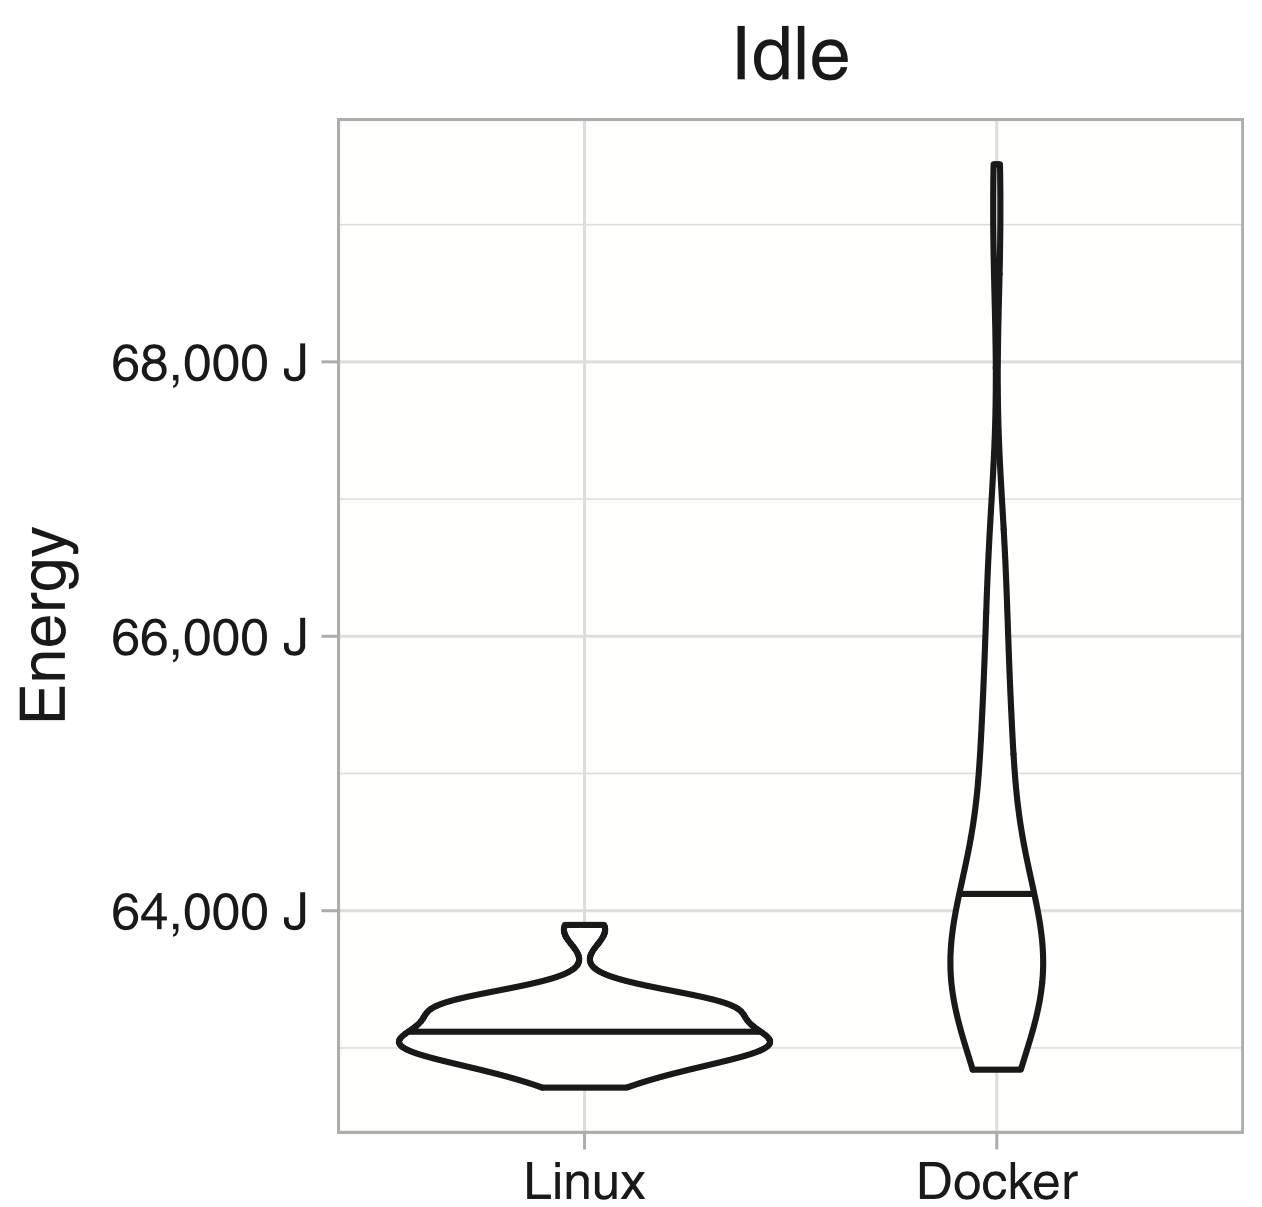
\includegraphics[width=.5\linewidth]{imgs/docker_vs_vm_energy_paper/idle_energy}}
    \caption{energy consumption of Idle system with and without docker \cite{santos2018does}}\label{fig:docker_idle}
\end{figure}

In the other hand, as one can see in Figure~\ref{fig:docker_reddis}.
Docker increased the execution time of the benchmark by 50 seconds, hence increasing the energy consumption.
The authors reported that this overhead is mostly due to the Docker deamon and not the fact that the application is in a container.
Moreover, they estimated the cost of this extra energy and it was less than 0.15\$ in the worst case, which is non-significant compared to the benefits that Docker brings for isolation and reproducibility.

To summarize, Docker-based software tends to consume more energy, because mainly they take more time to be executed.
The average power consumption is higher with only \textbf{2\,Watts}, due to the execution of the Docker deamon.
This overhead can reach up to 5\% for IO-intensive application, but it is merely noticeable when it comes to CPU- or DRMA-intesive workloads.

\begin{figure}
    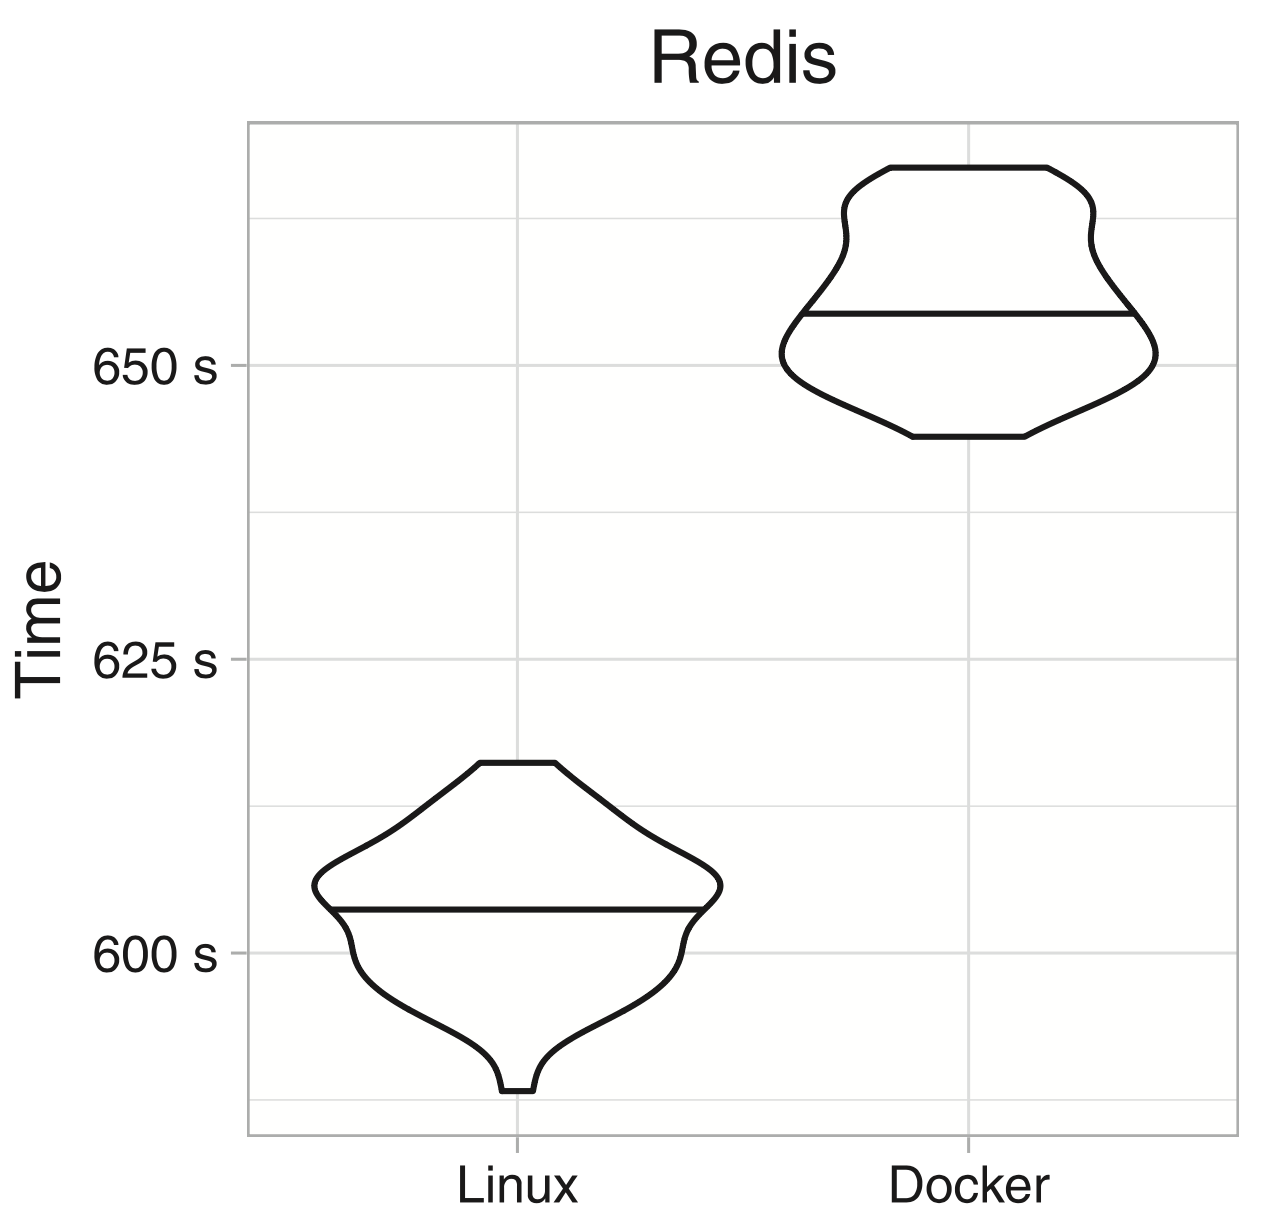
\includegraphics[width=.5\linewidth]{imgs/docker_vs_vm_energy_paper/reddis_time}
    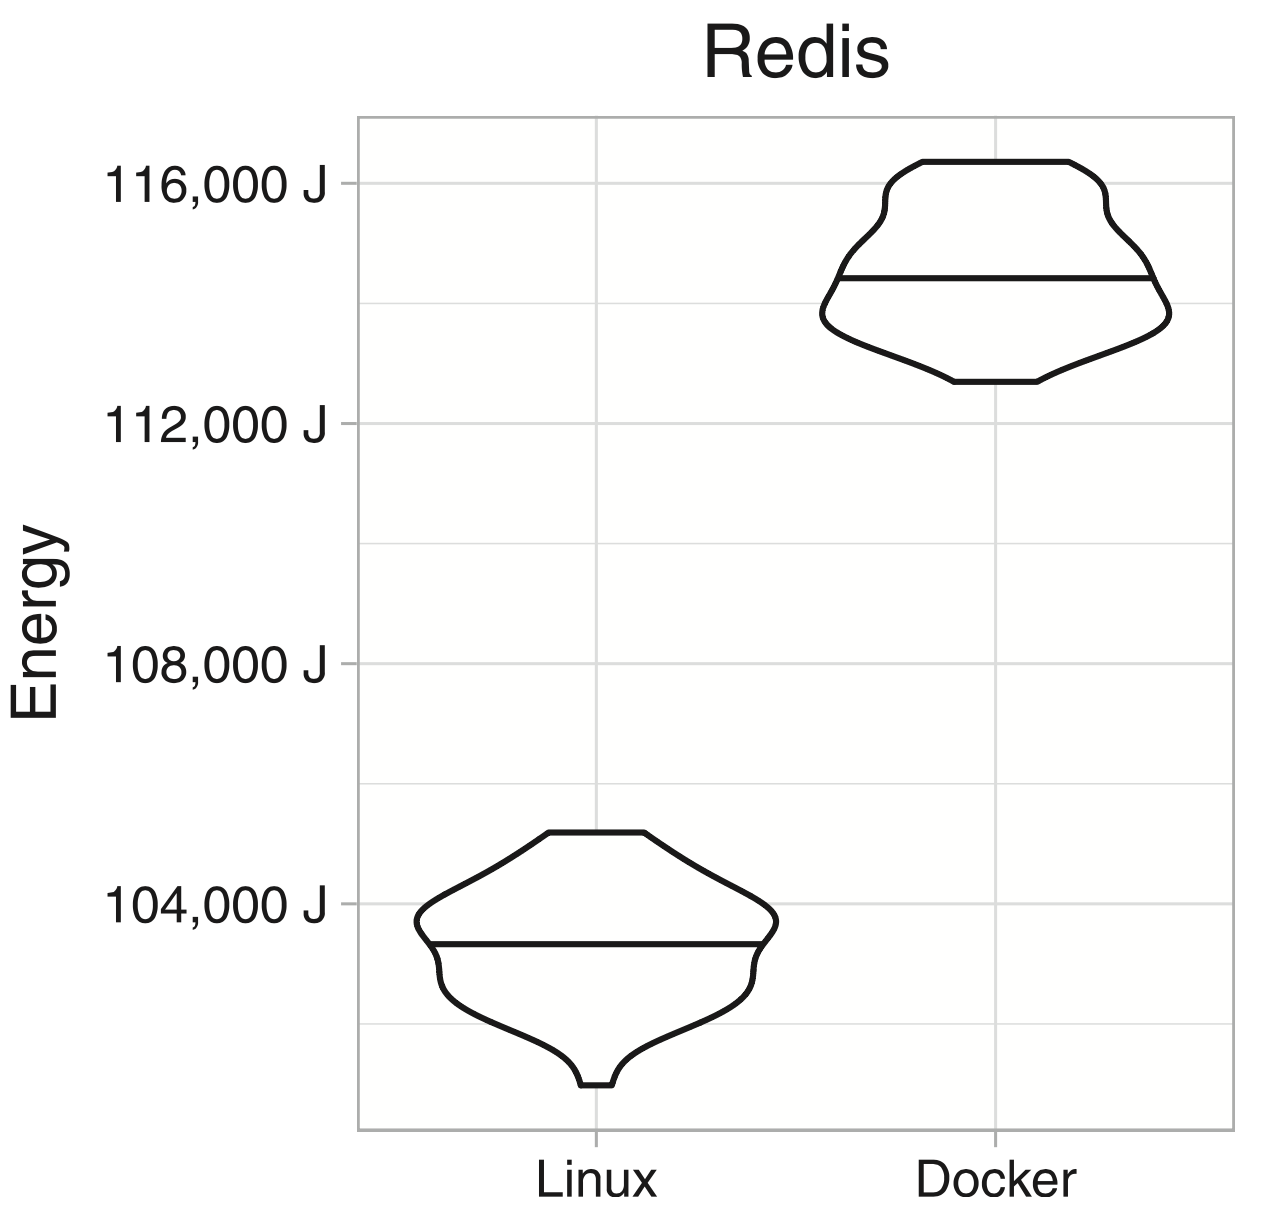
\includegraphics[width=.5\linewidth]{imgs/docker_vs_vm_energy_paper/reddis_energy}
    \caption{Execution time \& energy consumption of Redis with and without Docker~\cite{santos2018does}}\label{fig:docker_reddis}
\end{figure}


\subsection{Conclusion}
As one can see, Docker impact on energy is more constat due to the introduction of the supervisor. which will be applied to all the experimenets evenly. Therefore when it comes to comparison analysis, it will mitigate its impact autimatically. 
Moreover since we have access to the host Hardware, we dont have to worry about catching the energy consumption for the SUT. 
Therefore we will be conducting all our experiments using docker as an encapsuation technology. wich will ensure the reproducibility of our experiments with a simple and easy way. 